\documentclass[a4paper,titlepage]{report}

%PACKAGES
\usepackage[utf8]{inputenc}
\usepackage[T1]{fontenc}
\usepackage[francais]{babel}
\usepackage{amsmath}
\usepackage{amssymb}
\usepackage{mathrsfs}
\usepackage{fancyhdr}
\usepackage{lmodern}
\usepackage{graphicx}
\usepackage{geometry}
\usepackage{fancybox}
\usepackage{textcomp}
\usepackage{subfigure}

%Symbole euro
\usepackage{eurosym}

%Listings : affichage code
\usepackage{listings}


%Elements de la page de garde
\begin{document}

\begin{titlepage}

\begin{figure}
\centering

\includegraphics[width=5cm]{logo-ulg.png}
\end{figure}



\title{
\vspace{0.2cm}
\LARGE{\textbf{Projet 1 - Chaînes de Markov}} \\ \textsc{Eléments de processus stochastiques}
\author{\textbf{Floriane Magera} \\ \textbf{Romain Mormont} \\ \textbf{Fabrice Servais}\\ Troisième bachelier en sciences de l'ingénieur}
\date{}
\rule{15cm}{1.5pt}
}

%\geometry{hmargin=2.5cm}
\end{titlepage}

%DOCUMENT
\pagestyle{fancy}
\lhead{Projet 1 - Chaînes de Markov}
\rhead{Éléments de processus stochastiques}

%Page de garde
\maketitle

\newpage
\chapter{Question 1}
\section{Etude du modèle de base}
\paragraph{2)} Avant de calculer cette matrice, il est nécessaire de définir les poids/probabilités que nous appliquerons aux arcs du graphe modélisant la partie du Web qui nous intéresse. Nous avons décidé que la répartition des probabilités sur les arcs quittant un noeud doivent être uniforme (toutes les transitions sont donc équiprobables). 
\paragraph{}
Suite à ce choix, la formation de la matrice de transition est très simple. Si l'on note $A$ la matrice d'adjacence, alors il suffit d'appliquer la formule suivante pour calculer l'élément Q(i,j) :
\[
Q(i,j) = A(i,j) \times \frac{1}{n}\sum\limits_{j = 1}^n A(i,j)
\]
Cette formule permet de placer à $0$ les éléments de $Q$ représentant une transition impossible et de placer à une certaine probabilité les autres éléments de $Q$.
\paragraph{3)} Nous avons choisi un nombre de pas $t = 20$. Le cas où le surfeur démarre aléatoirement sur le graphe est représenté par une distribution initiale $\pi_0$ uniforme et le cas où le surfeur démarre d'une page donnée est représenté par une distribution initiale $\pi_0$ où toutes les probabilités sont nulles sauf à l'index correspondant au noeud de départ. L'évolution des probabilités dans les deux cas est donnée sur le Figure \ref{fig:q113}.
\begin{figure}[h]
	\center
	\subfigure{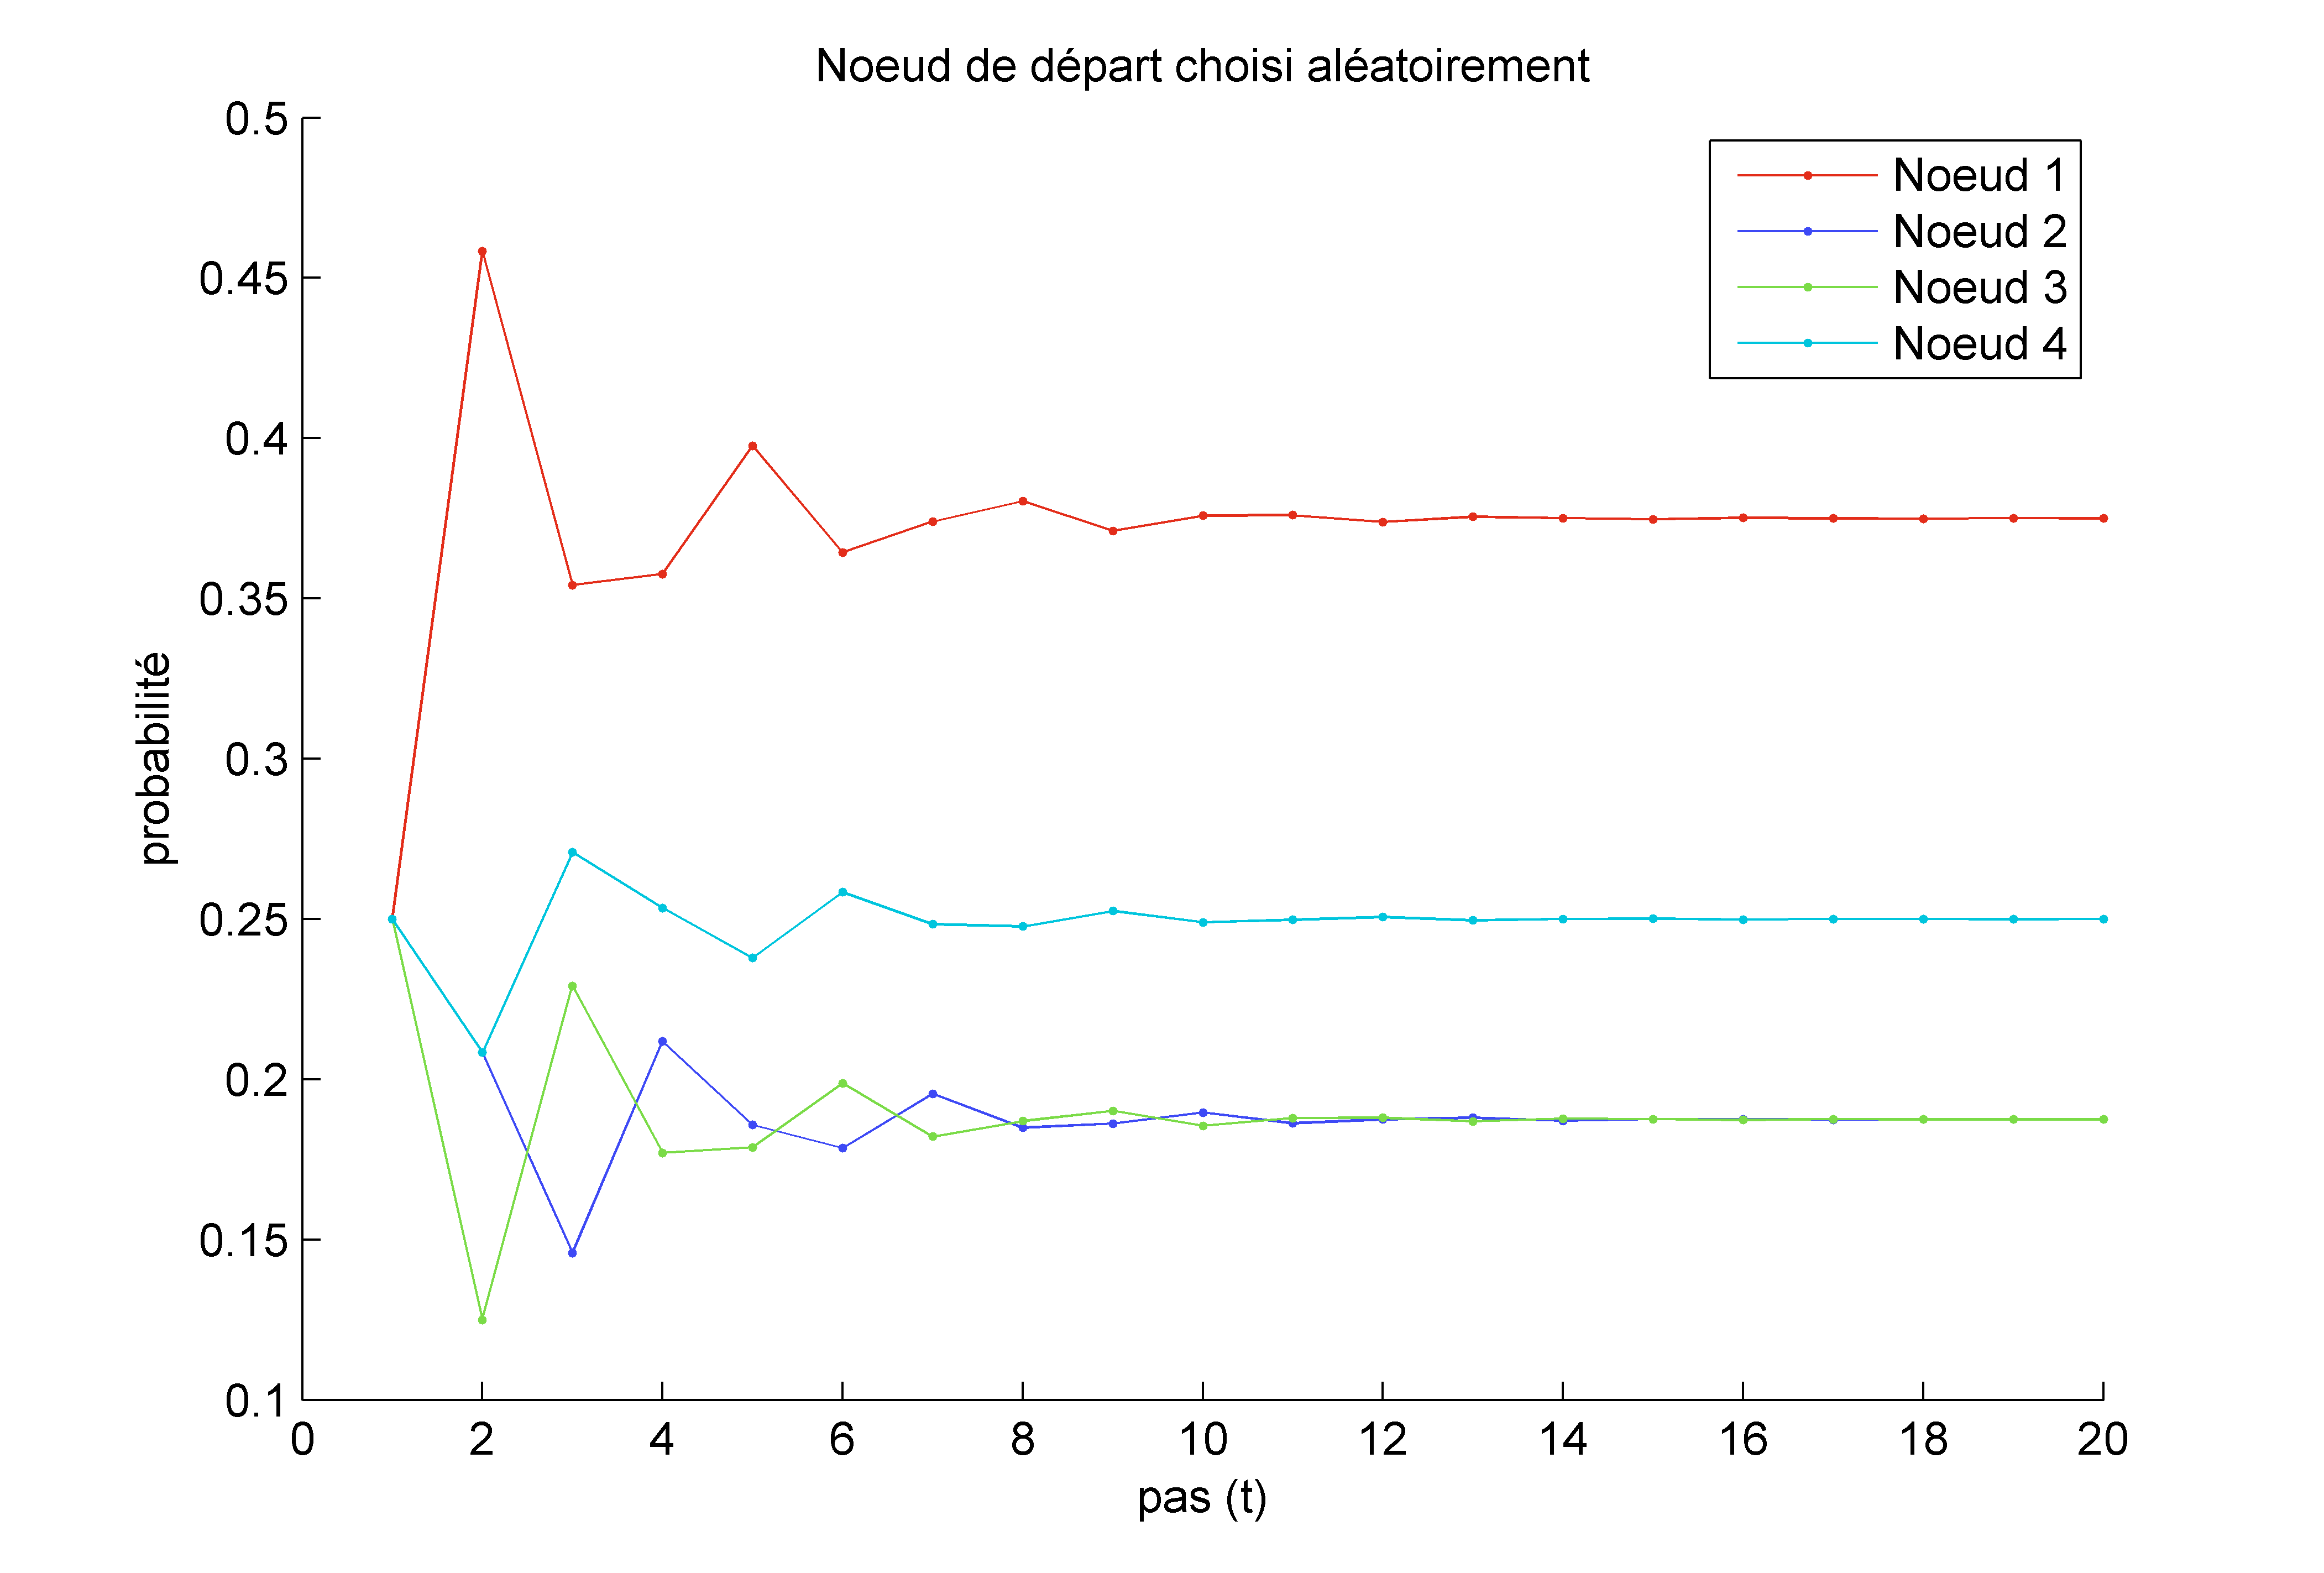
\includegraphics[scale=0.35]{../images/q1131_proba.png}}
	\subfigure{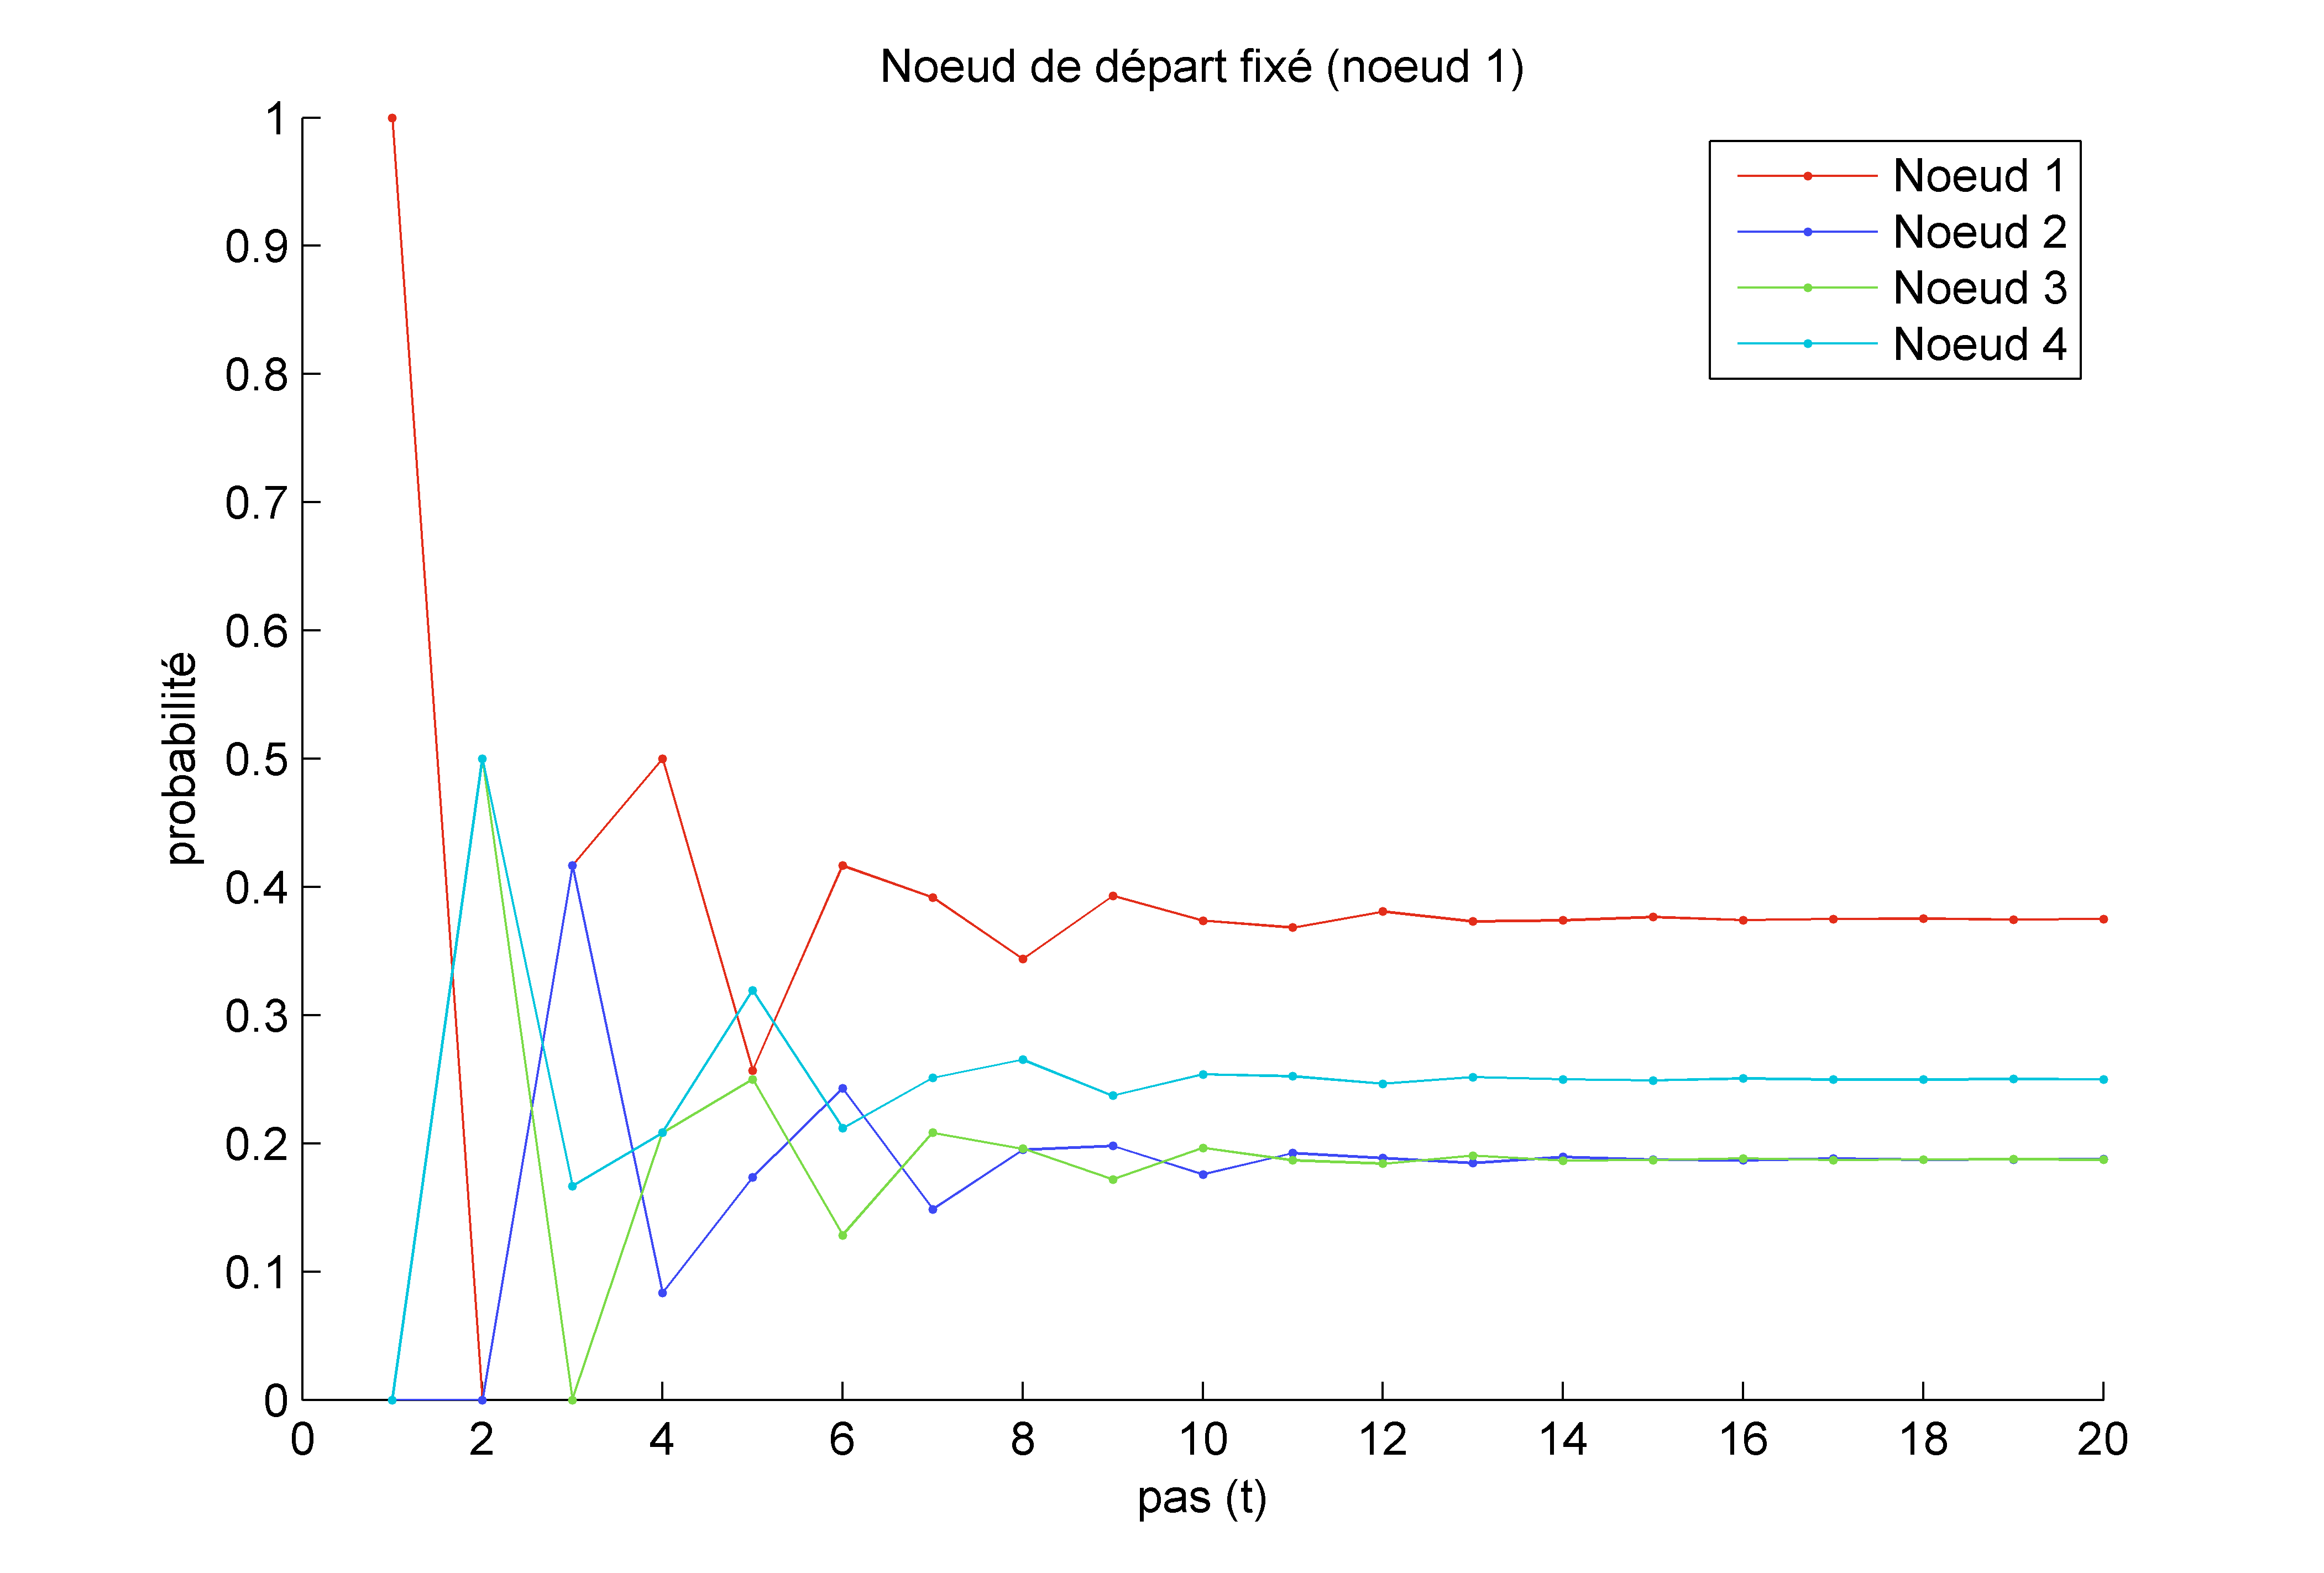
\includegraphics[scale=0.35]{../images/q1132_proba.png}}
	\caption{Évolution de la distribution de probabilité}
	\label{fig:q113}
\end{figure}
\paragraph{}
La matrice $Q^{(20)}$ obtenue est la suivante :
\[
Q^{(20)} = 
\begin{pmatrix}
 0.3751 & 0.1874 & 0.1875 & 0.2500\\
 0.3751 & 0.1877 & 0.1874 & 0.2499\\
 0.3749 & 0.1875 & 0.1875 & 0.2500\\
 0.3749 & 0.1875 & 0.1875 & 0.2500\\
\end{pmatrix}
\]
On constate une convergence des distributions de probabilités vers un distribution $\pi_s$ commune pour les deux distributions initiales ainsi qu'une convergence de la matrice $Q$. 
\paragraph{4)} La distribution stationnaire de la chaîne de Markov calculée par la méthode des puissances est la suivante :
\[
\pi_\infty = 
\begin{pmatrix}
0.3750 &
0.1875 &
0.1875 &
0.2500 \\
\end{pmatrix}
\]
\paragraph{5)} On constate que le noeud 1 possède le meilleur PageRank, suivi des noeuds 2 et 3 à égalité et du noeud 4. On peut expliquer ce classement intuitivement : 
\begin{itemize}
	\item le \textbf{noeud 1} possède le plus d'arêtes entrantes donc ayant le plus de chance d'être visité
	\item le \textbf{noeud 3} possède le moins d'arêtes entrantes donc ayant le moins de chance d'être visité
	\item les \textbf{noeuds 2} et \textbf{4} possèdent le même nombre intermédiaire (par rapport aux deux autres) d'arêtes entrantes. Le PageRank du noeud 4 est néanmoins plus élevé que celui du noeud 2 puisque le noeud 4 possèdent une arête entrante venant du noeud 1 qui est le plus visité.
	\item malgré un nombre d'arête entrante plus élevé que pour le noeud 3, le \textbf{noeud 2} possède une PageRank égal. Cela est dû au fait que, d'une part, le noeud 3 peut être visité depuis le noeud le plus visité (noeud 1) ce qui améliore son PageRank et, d'autre part, que le noeud 2 ne peut être accéder depuis des noeuds moins visités (noeud 3 et 4) ce qui abaisse son PageRank. 
\end{itemize} 
\paragraph{6)} Dans un premier temps, nous avons généré une chaîne pour chaque longueur. Le résultat obtenu est donné sur la Figure \ref{sfig:q116_evol_1}. On peut déjà observer que les différentes courbes obtenues oscillent autour de leur probabilité stationnaire associée. Néanmoins, le résultat nous semblant trop incertain étant donné les oscillations, nous avons décidé de refaire l'expérience en générant cette fois-ci 1000 chaînes pour chaque longueur (voir Figure \ref{sfig:q116_evol_2}). Nous avons ensuite moyenné afin d'obtenir un résultat exploitable. Les courbes obtenues nous permettent de confirmer les premières observations.
\begin{figure}[h]
	\center
	\subfigure[1 génération]{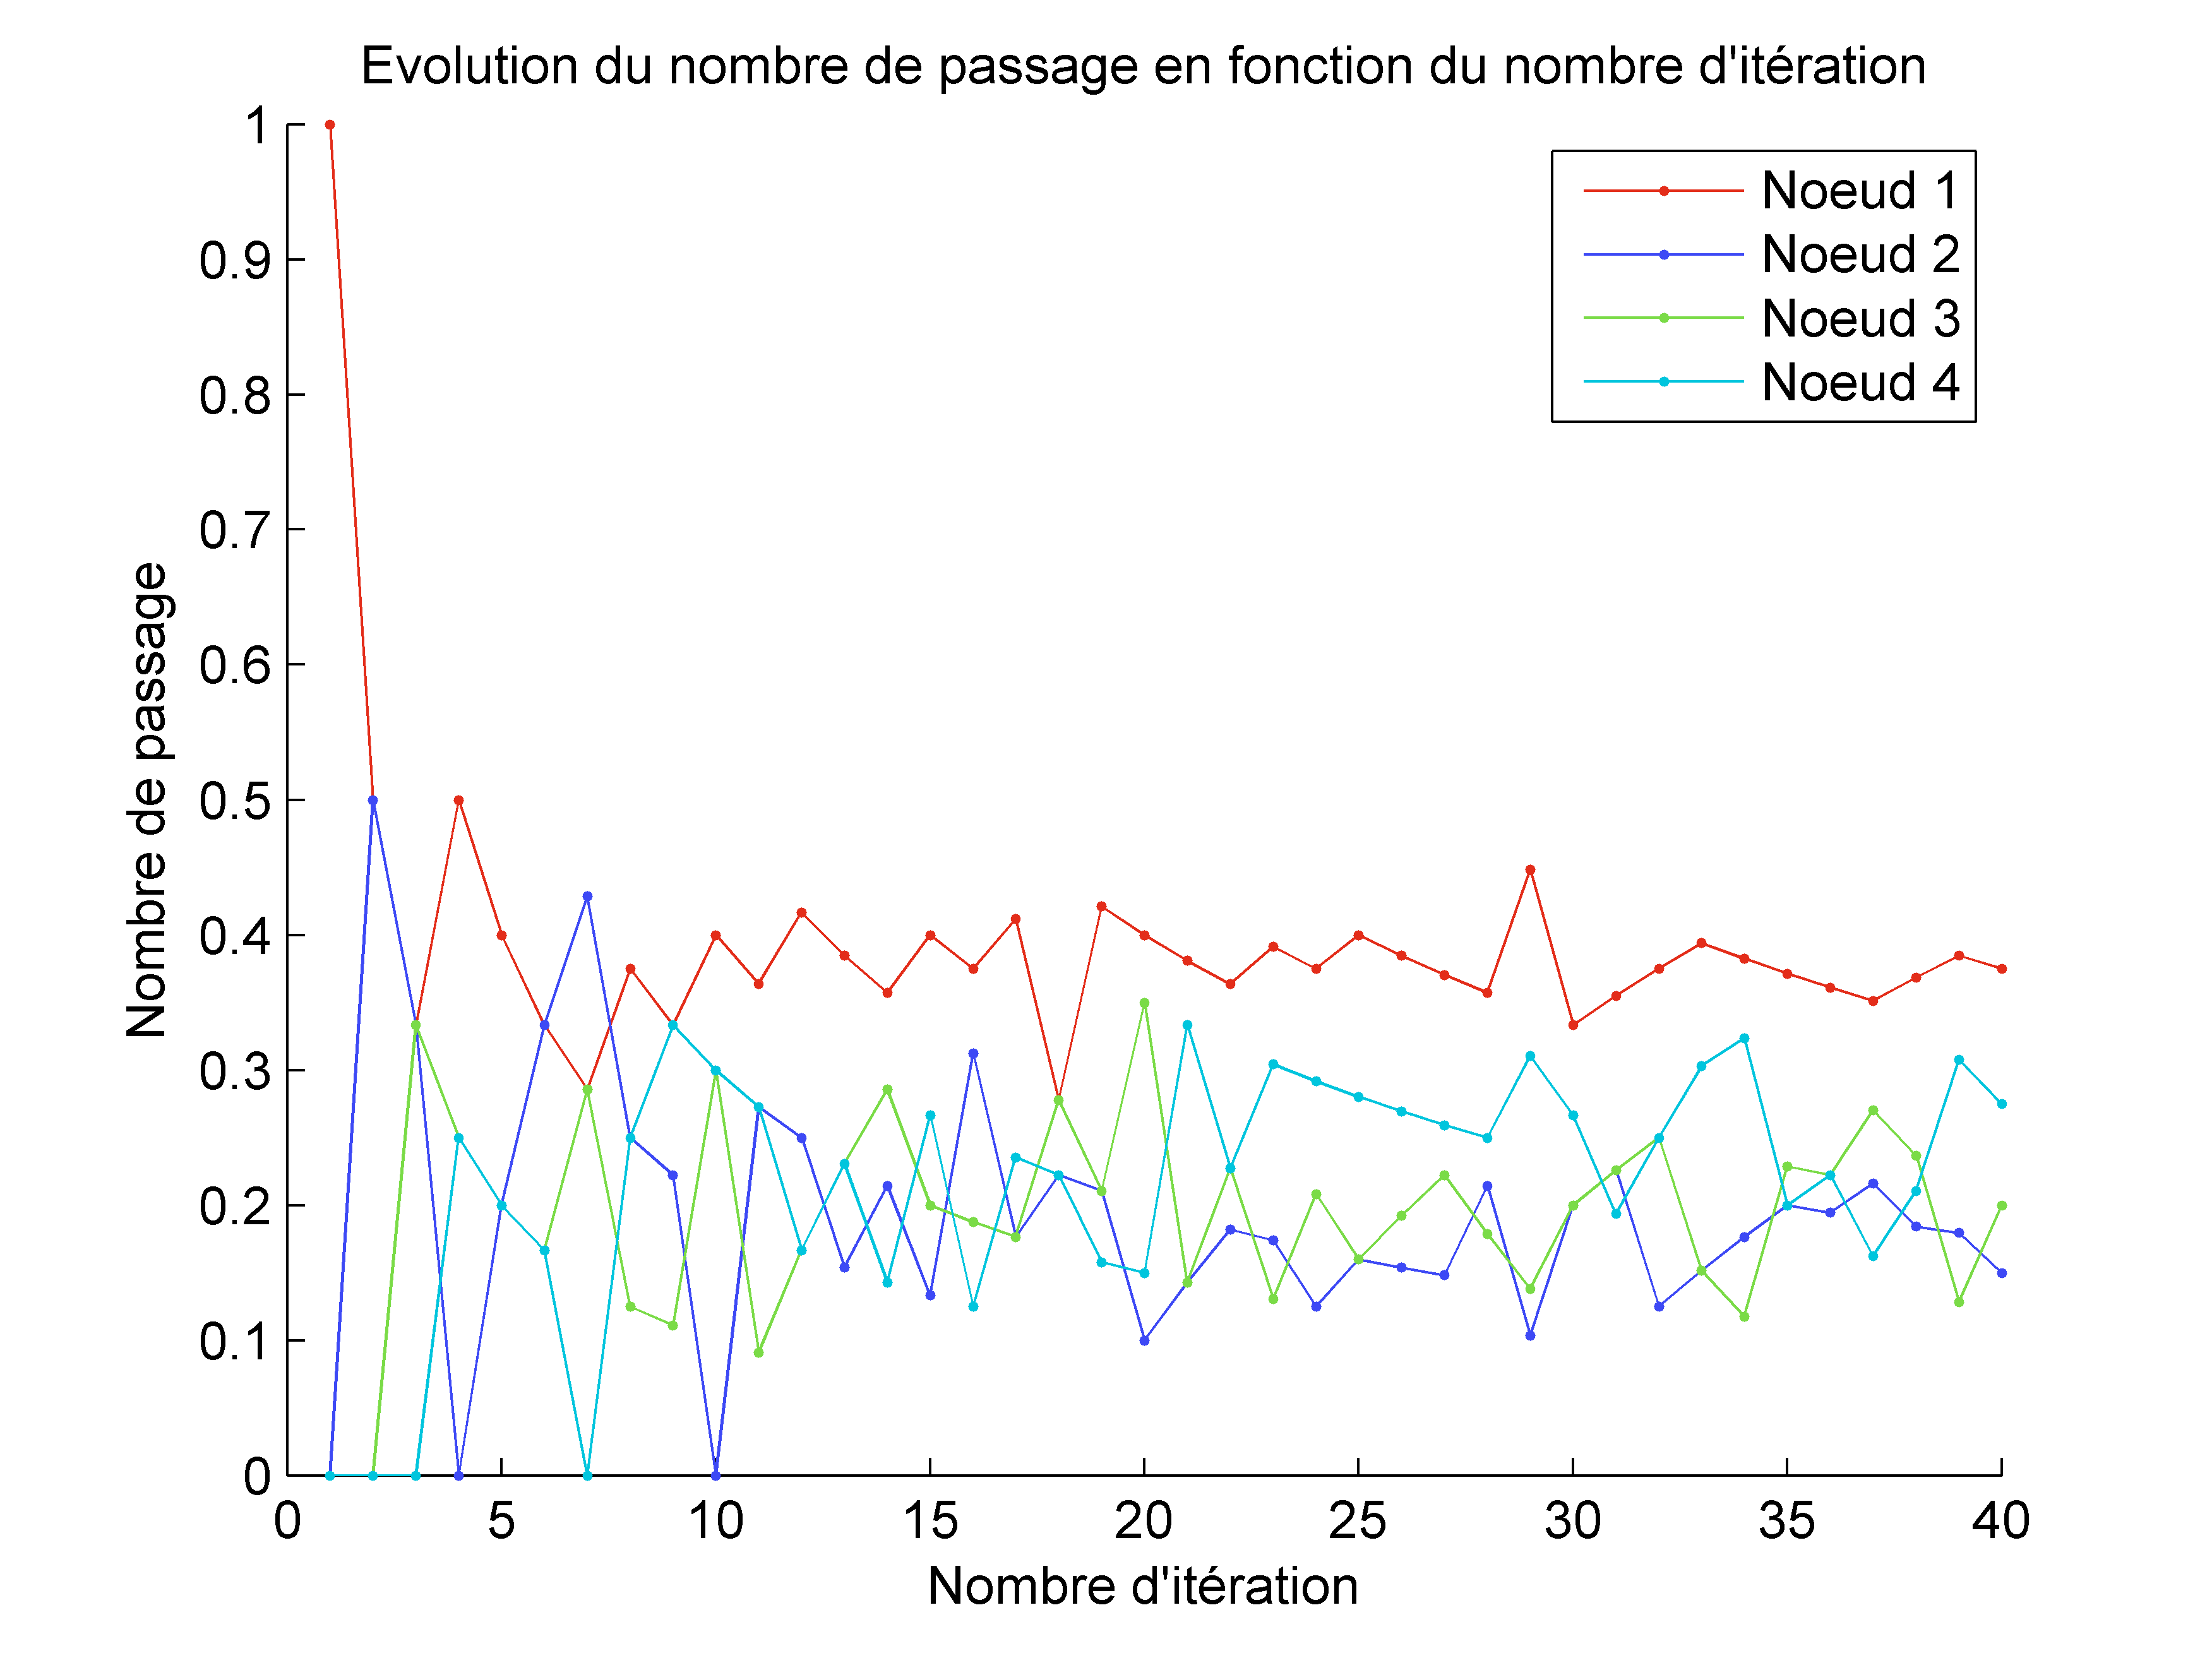
\includegraphics[scale=0.45]{../images/q116_evol_1.png}\label{sfig:q116_evol_1}}
	\subfigure[1000 générations]{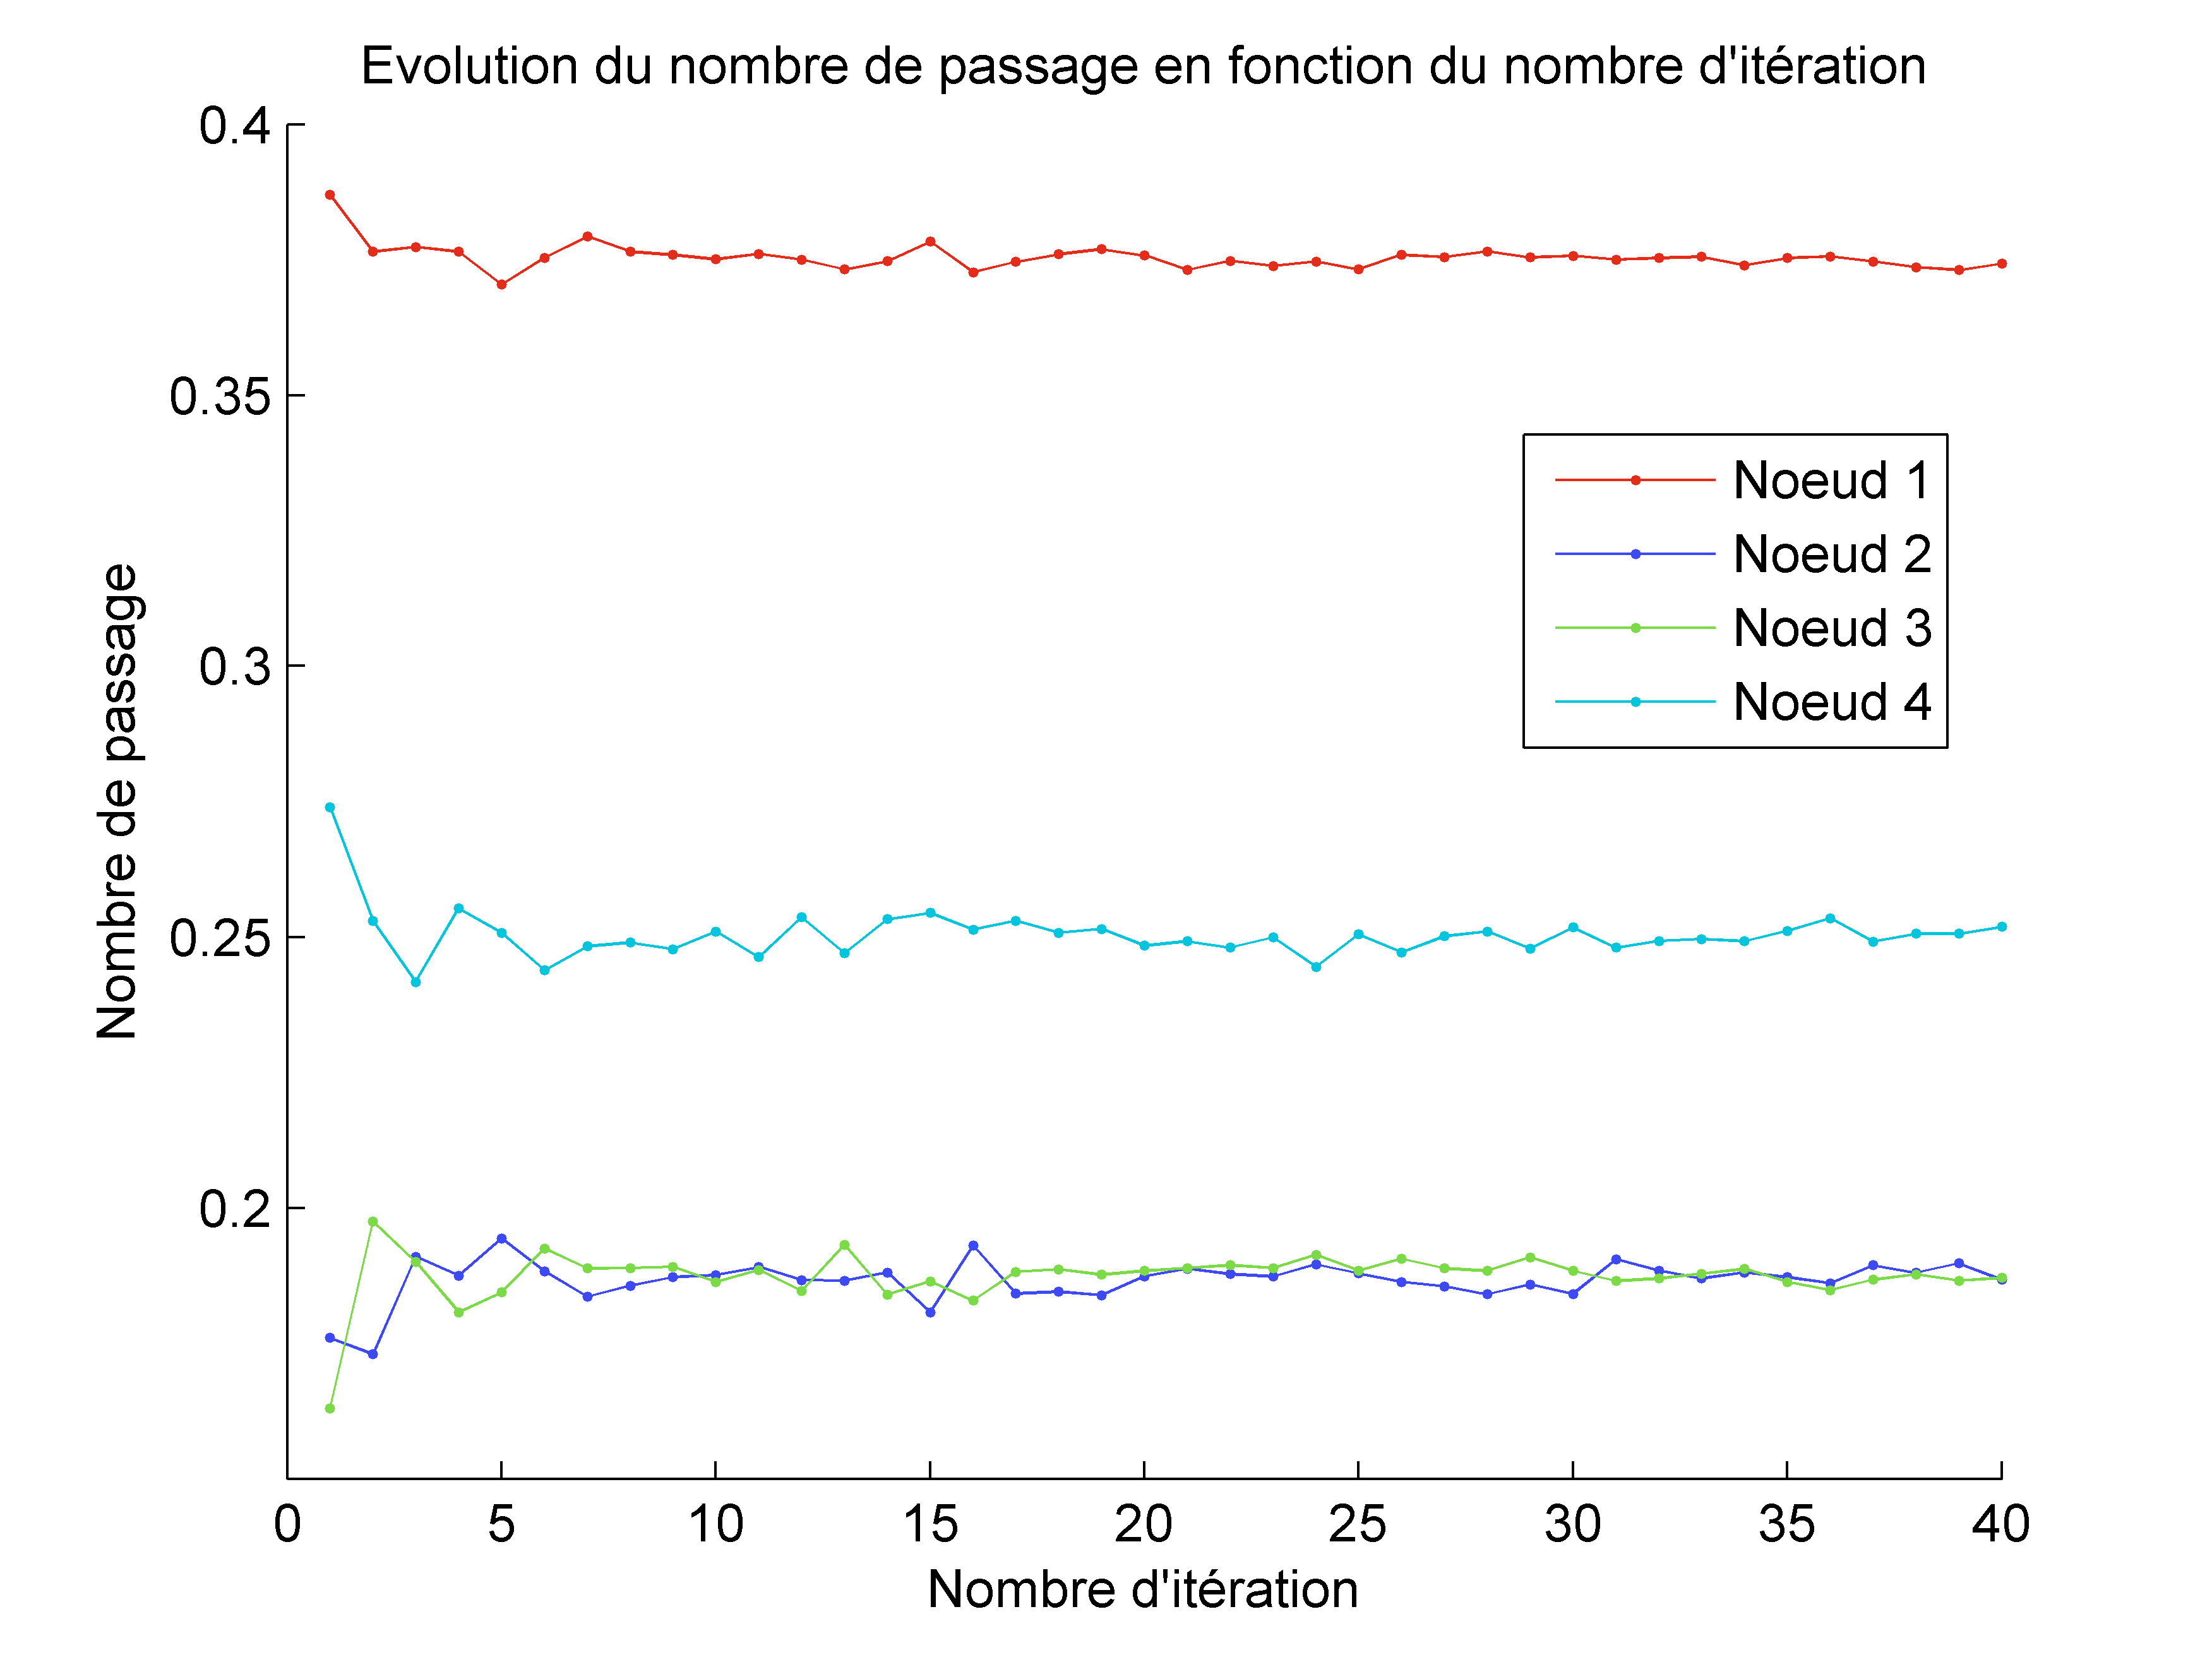
\includegraphics[scale=0.45]{../images/q116_evol_2.png}\label{sfig:q116_evol_2}}
	\caption{Évolution du nombre de passage par un noeud}
\end{figure}
\paragraph{7)} 
\subsection{Analyse des matrices $A_2$ et $A_3$}
\paragraph{1)} Les évolutions des distributions de probabilité sont données dans la Figure \ref{fig:q118}. On constate d'un part l'apparition d'\textbf{oscillations} et d'autre part que la \textbf{probabilité d'aller sur un certain noeud} (noeud 3 pour les deux matrices) devient \textbf{nulle} à partir d'un moment donné. 
\begin{figure}[h]
	\center
	\subfigure[Distribution initiale uniforme]{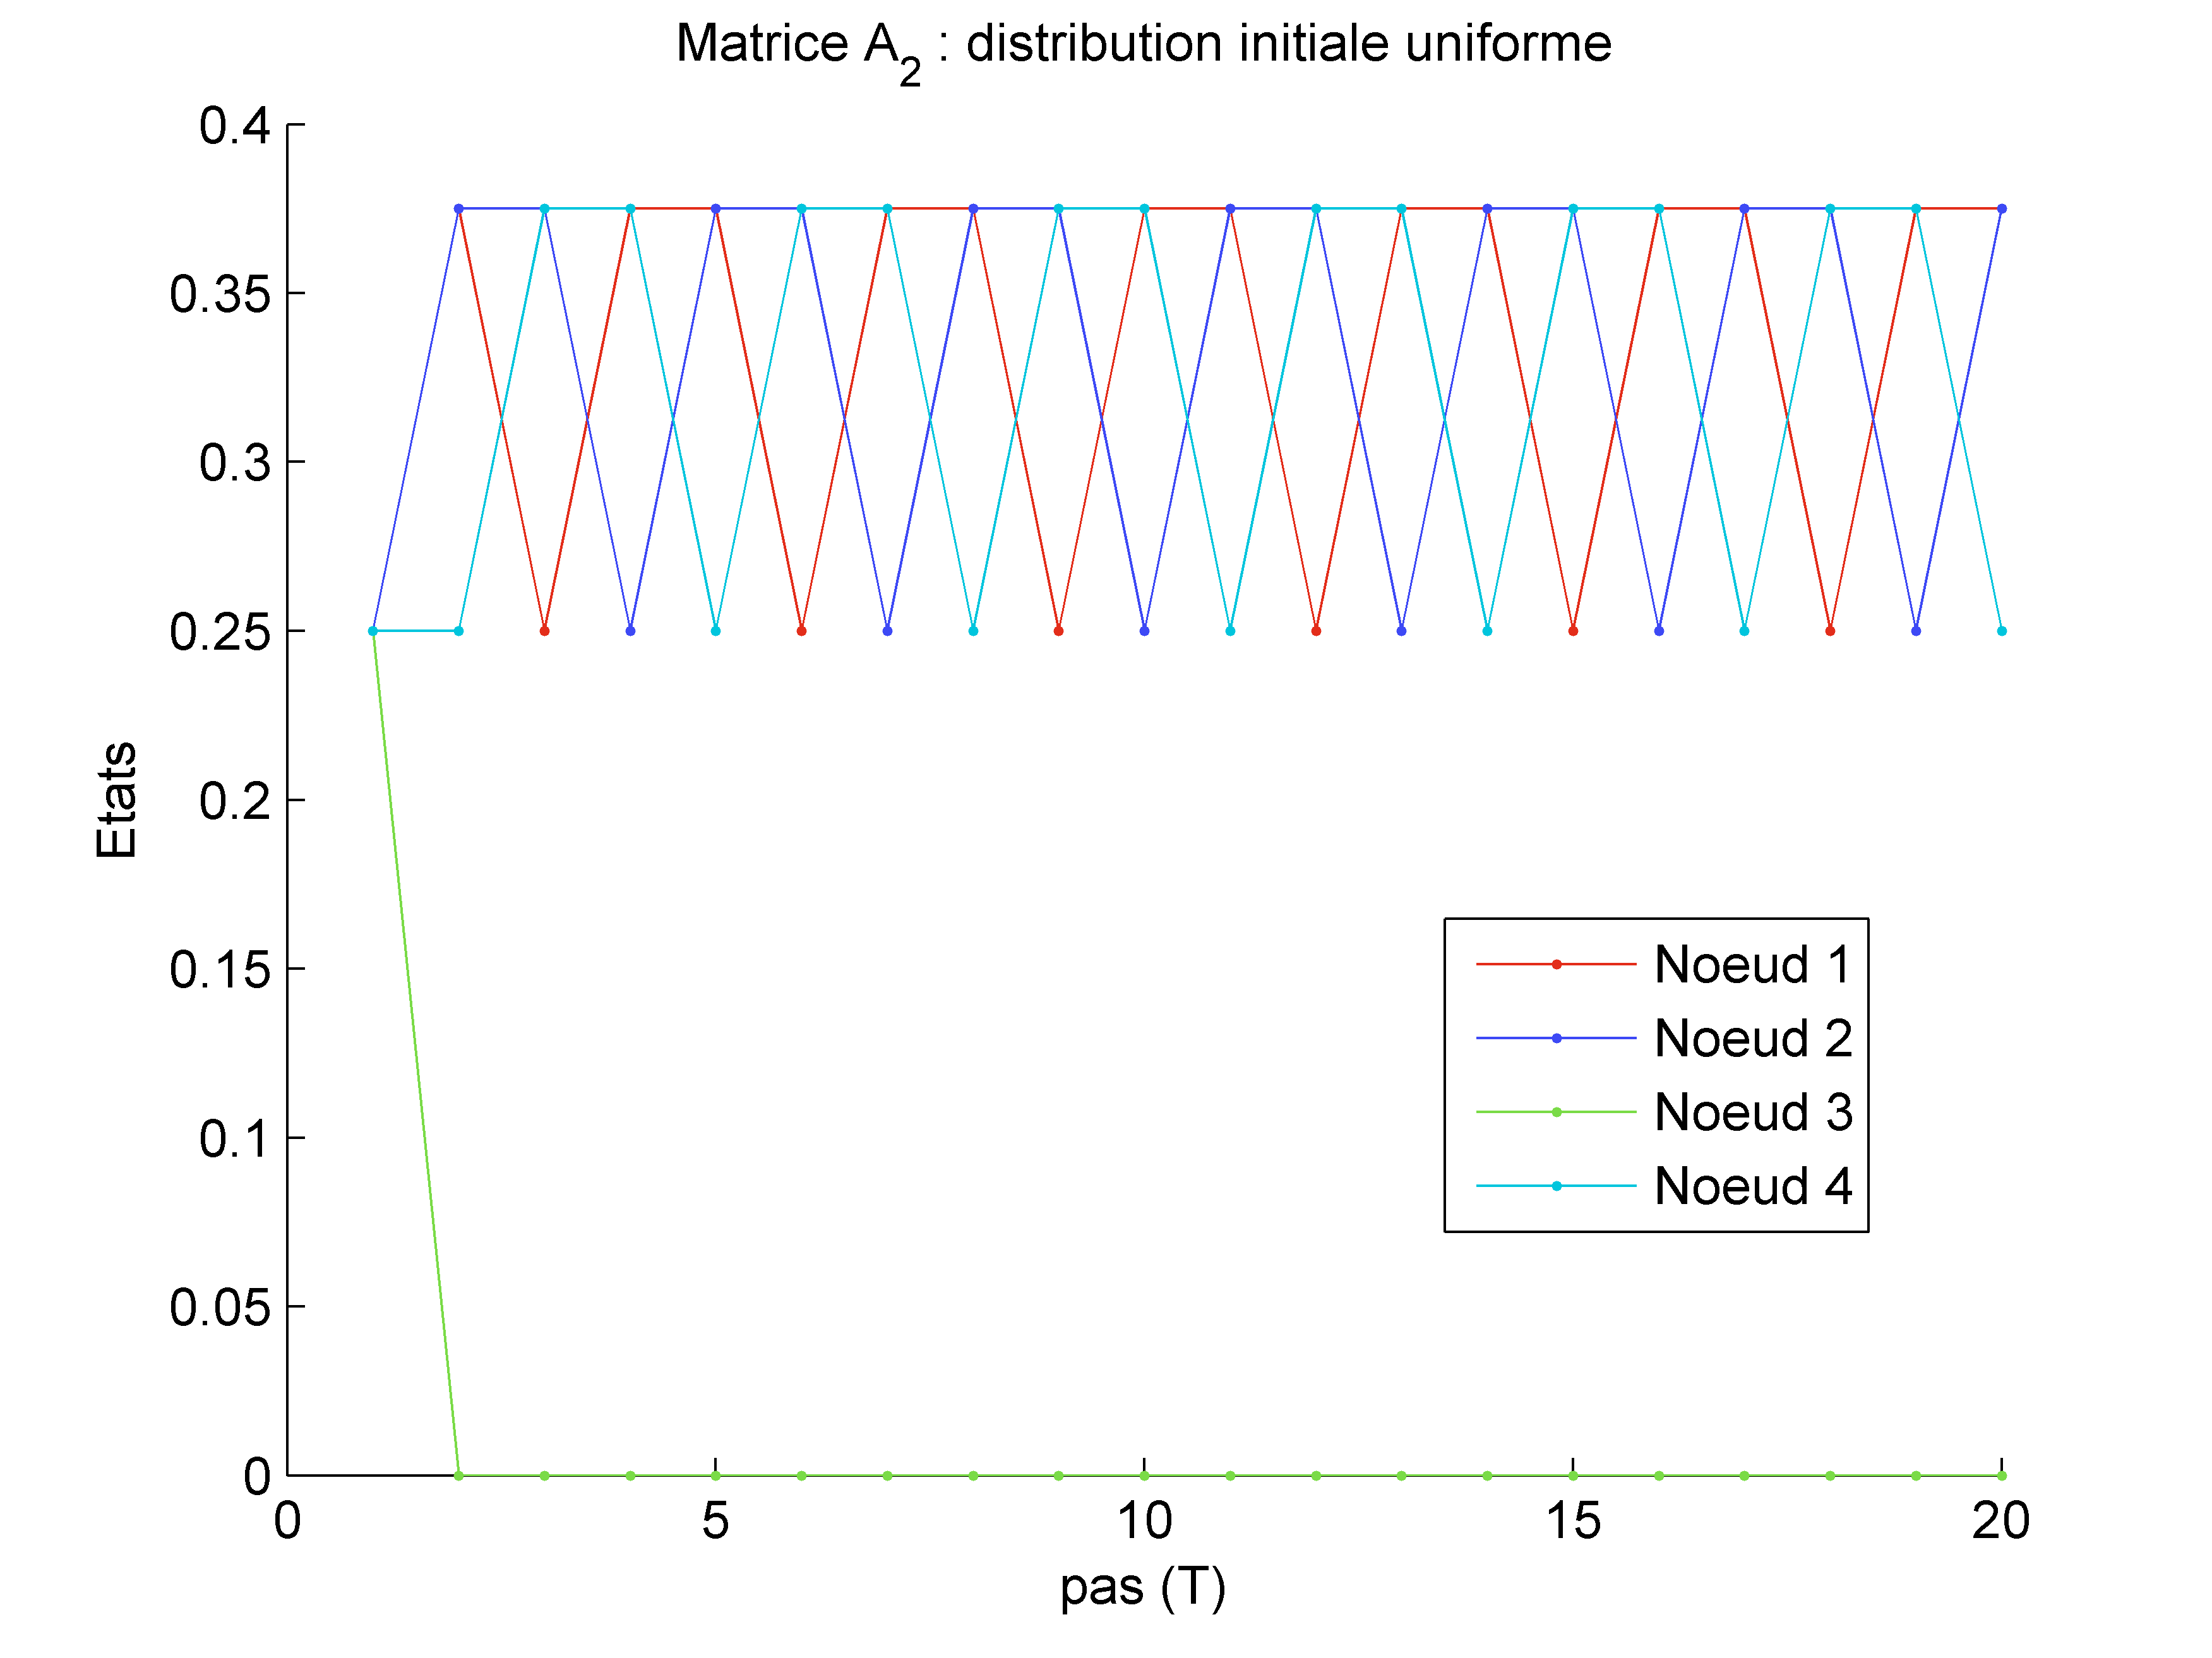
\includegraphics[scale=0.45]{../images/q118_evol_21.png}\label{sfig:q118_evol}}
	\subfigure[Depuis le noeud 1]{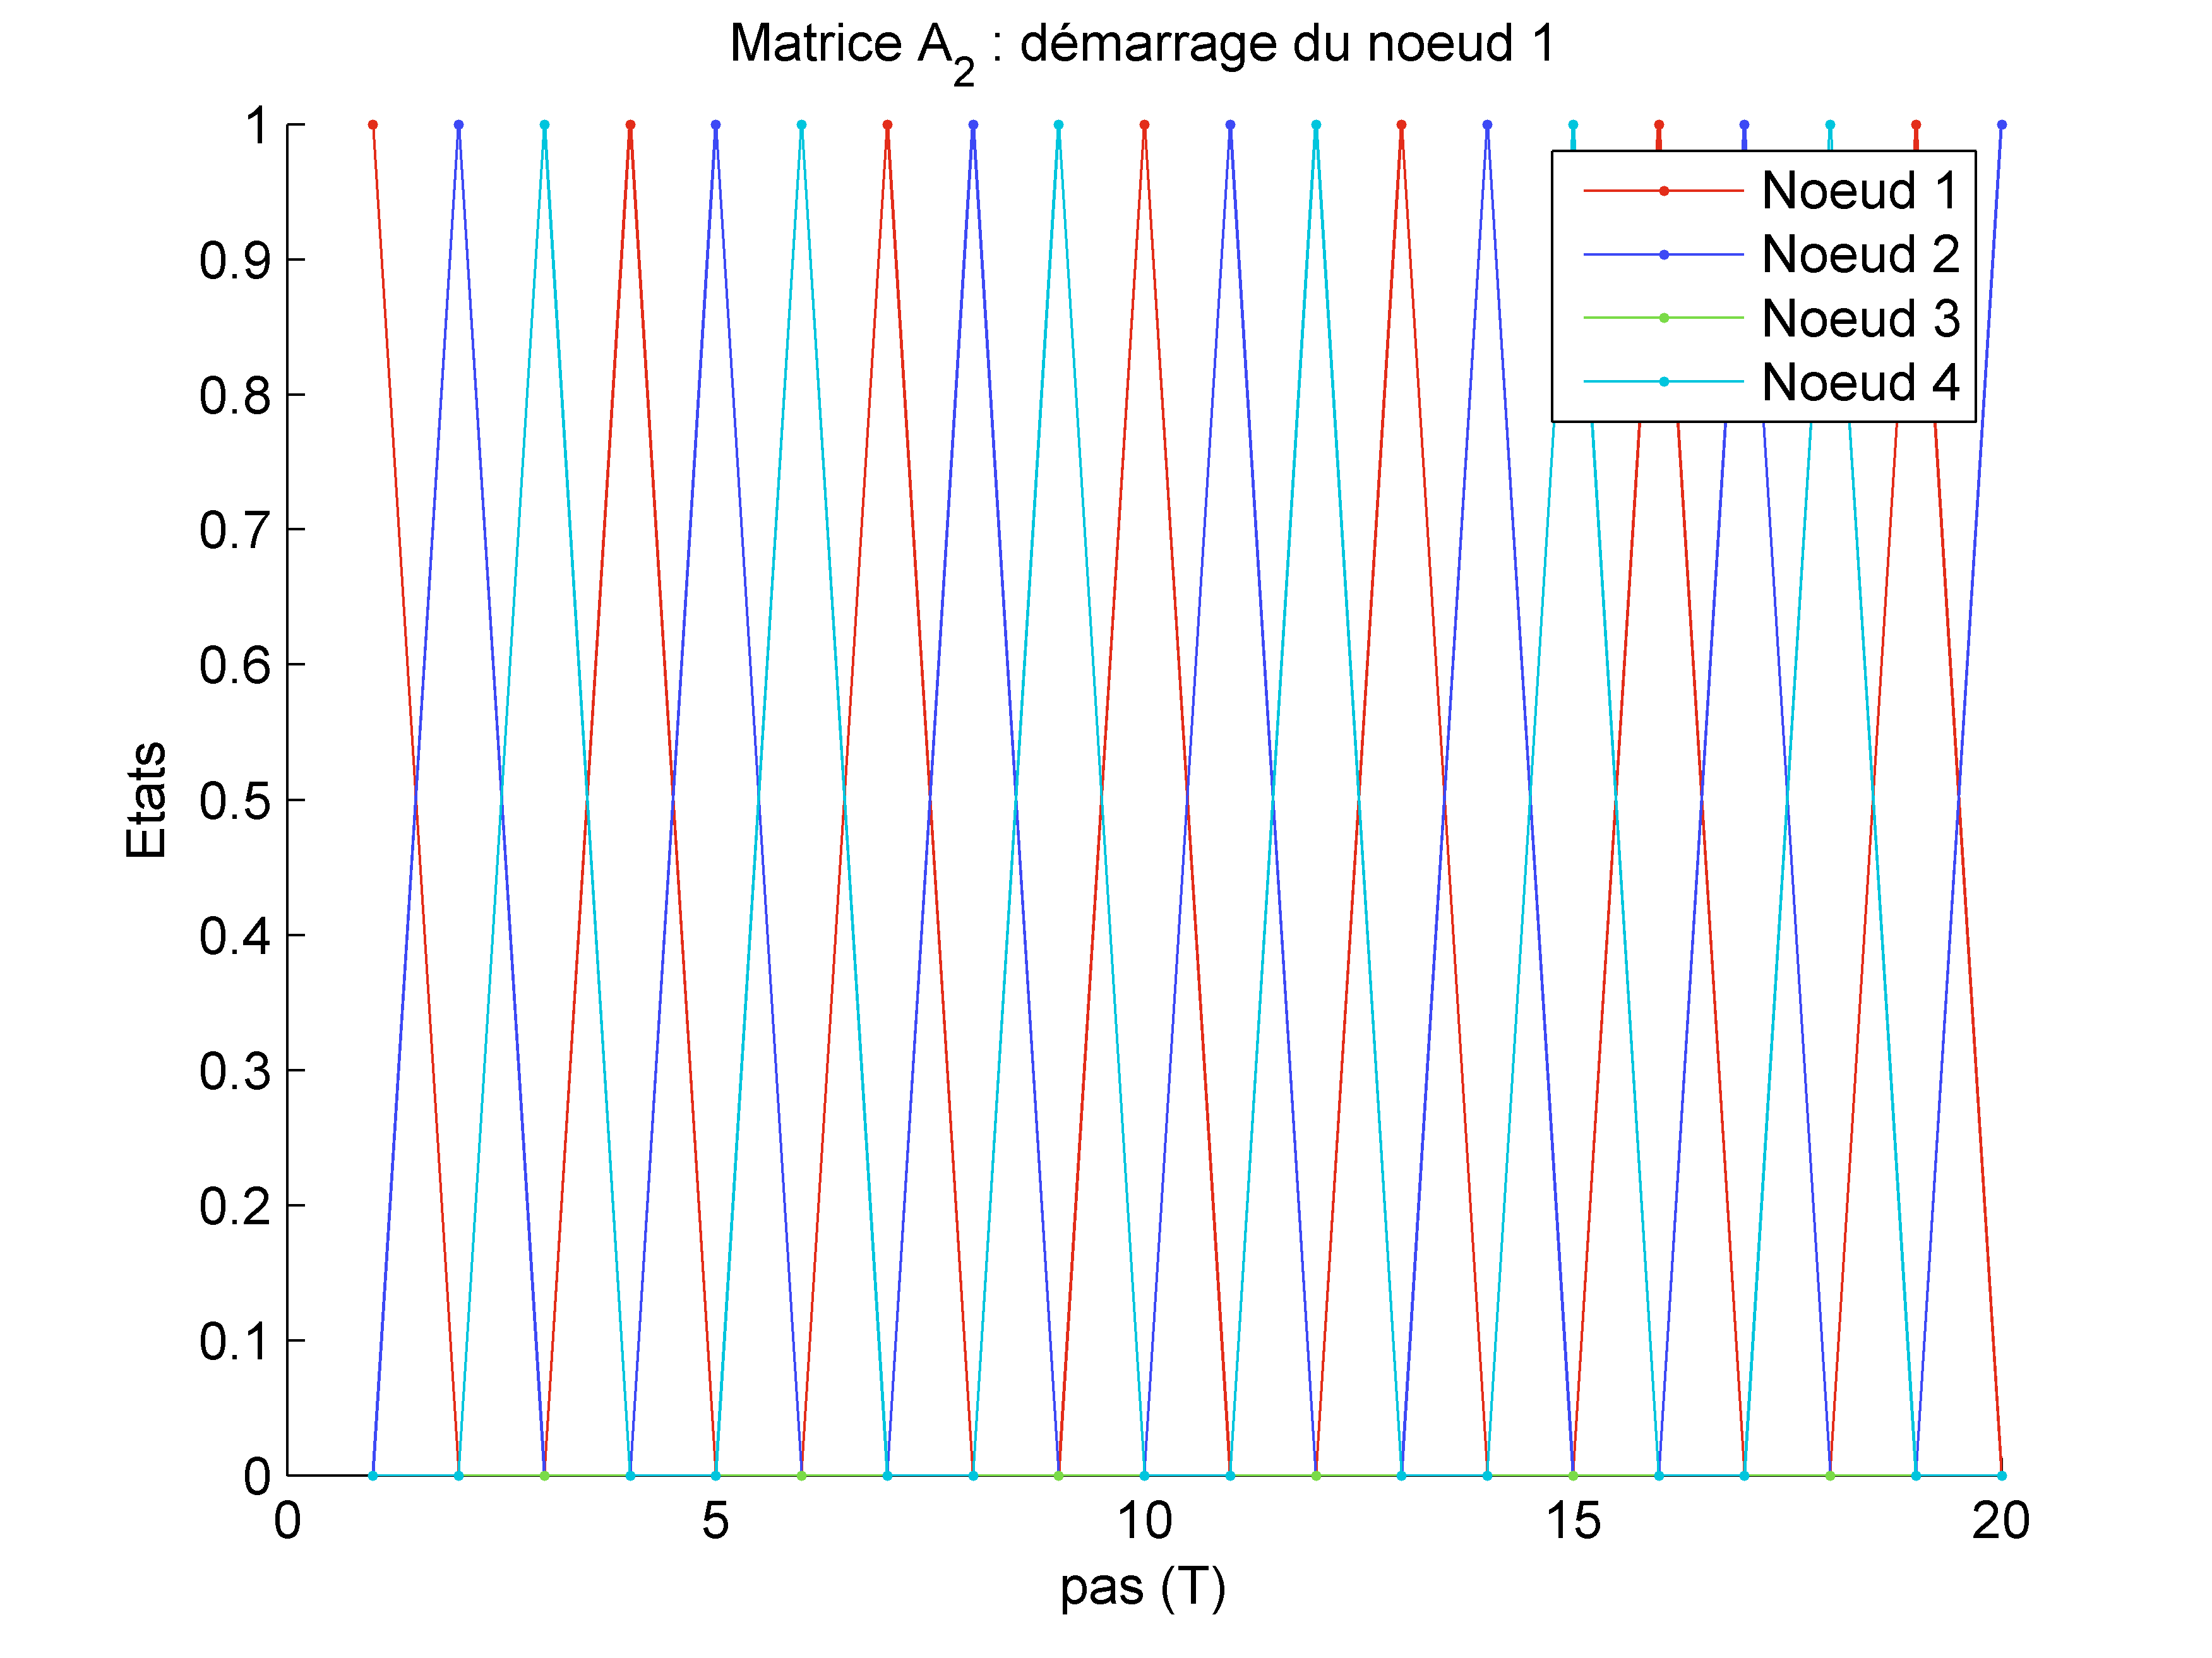
\includegraphics[scale=0.45]{../images/q118_evol_22.png}\label{sfig:q118_evol}}
	\subfigure[Distribution initiale uniforme]{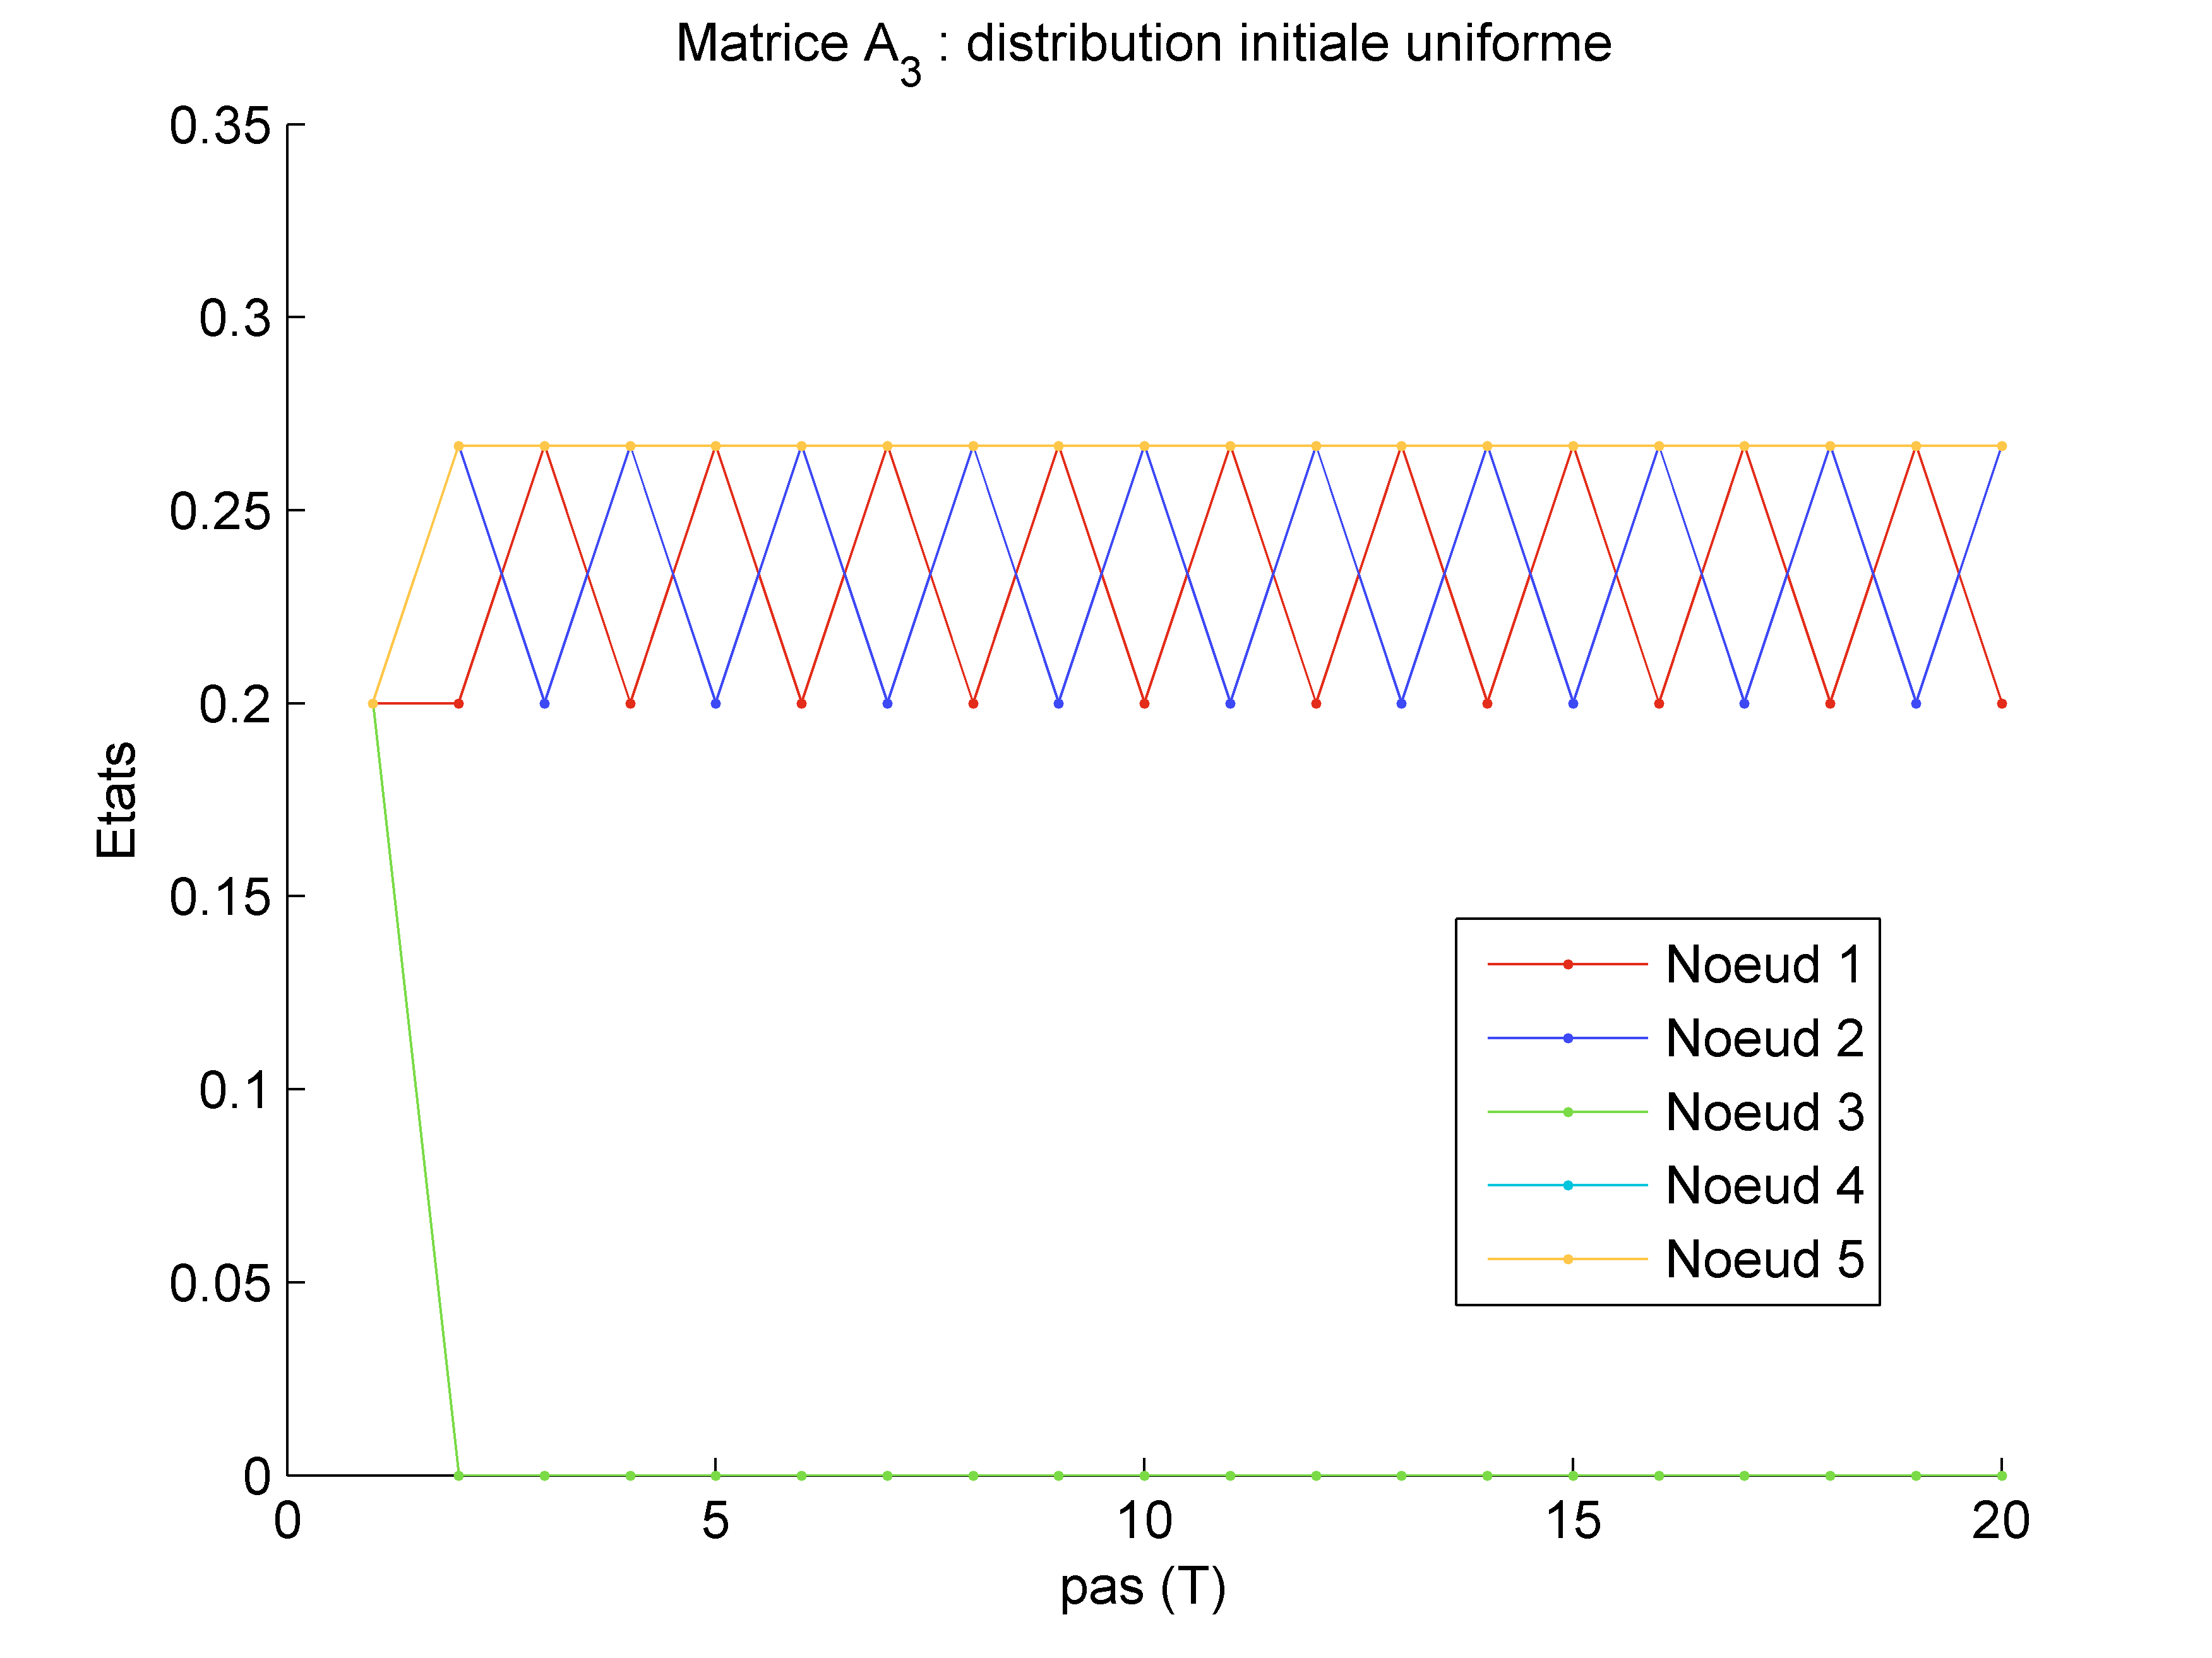
\includegraphics[scale=0.45]{../images/q118_evol_31.png}\label{sfig:q118_evol}}
	\subfigure[Depuis le noeud 1]{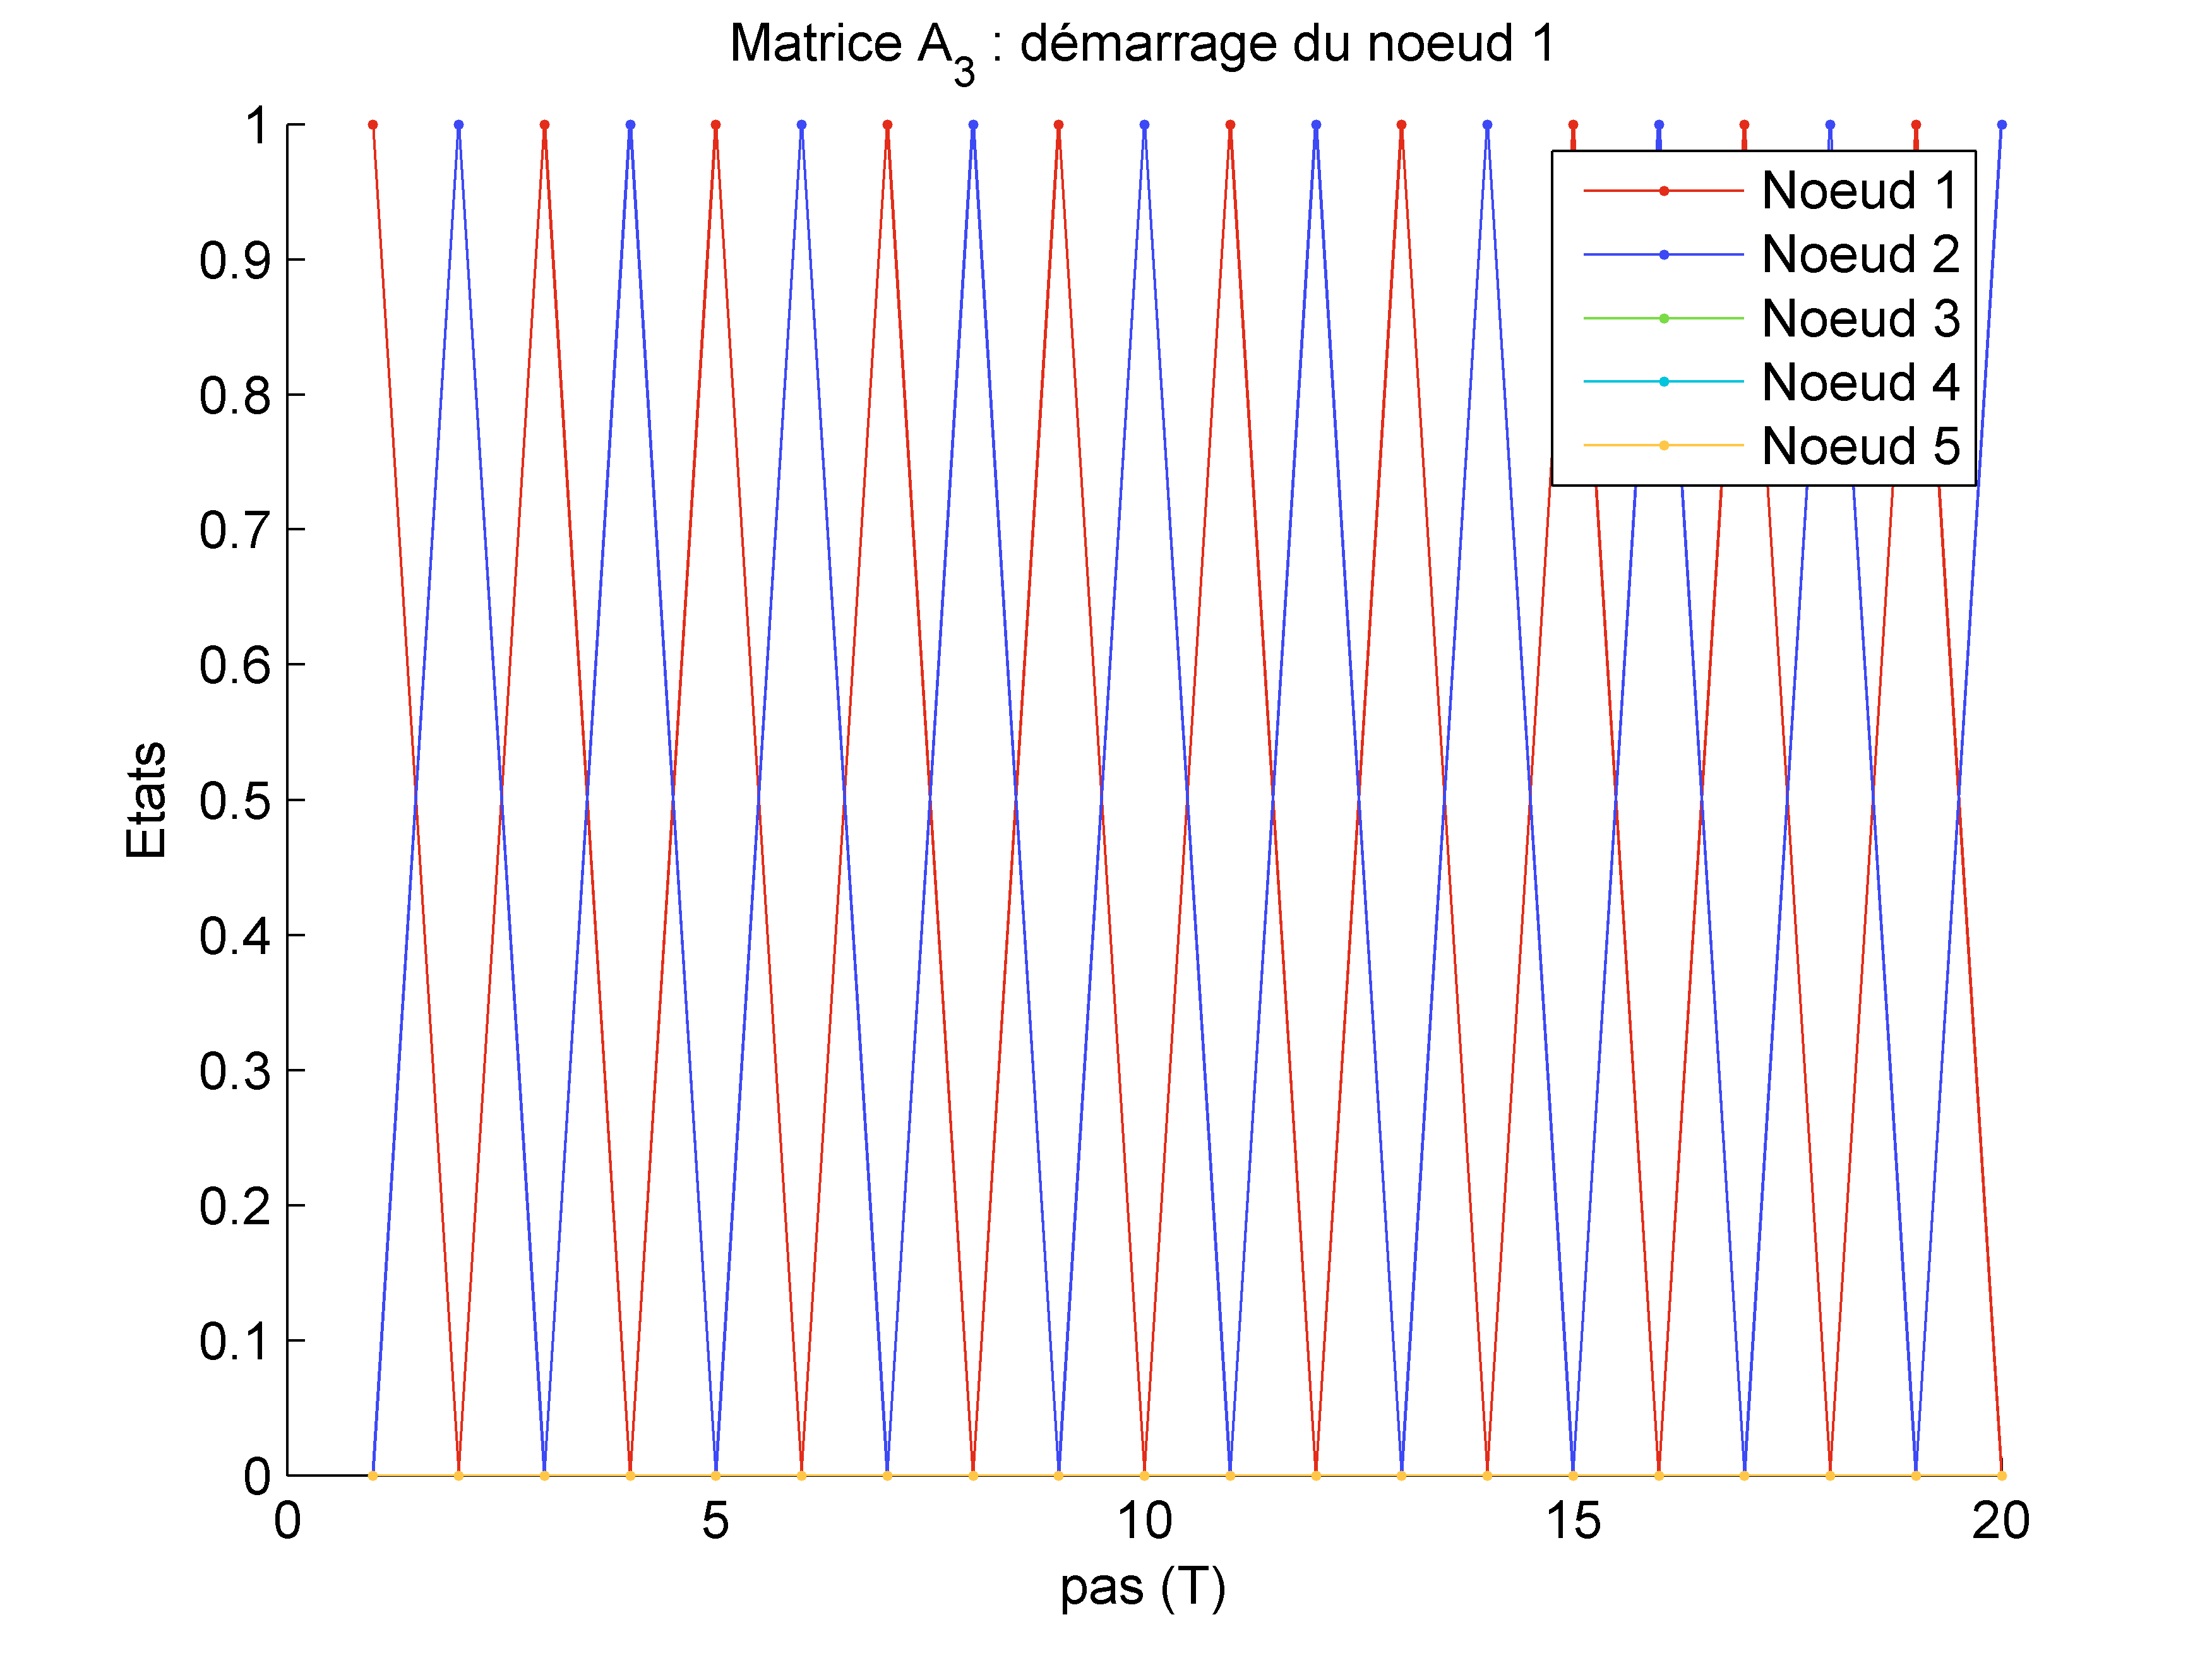
\includegraphics[scale=0.45]{../images/q118_evol_32.png}\label{sfig:q118_evol}}
	\caption{Évolution des distributions de probabilités}
	\label{fig:q118}
\end{figure}
\paragraph{2)} 
\section{Téléportation}
\paragraph{1)}
La formule utilisée pour calculer la matrice de transition $Q_t$ du modèle du surfeur avec téléportation est la suivante :
\[
	Q_t = (1 - \alpha) Q' + \alpha \tilde{Q}
\]
où $Q'$ et $\tilde{Q}$ sont des matrices de transition et $\alpha$ la probabilité de téléportation. 
\paragraph{}
La première est la matrice de transition du graphe initial auquel on a rajouté des arêtes partant des \textit{dangling nodes}. Elle a été calculée en remplaçant tous les éléments de la matrice $Q$ dans des lignes ne contenant que des 0 par $\frac{1}{n}$. Cette valeur $\frac{1}{n}$ a été choisie en considérant une densité de probabilité uniforme entre les différentes arêtes partant des \textit{dangling nodes}. 
\paragraph{}
La seconde est la matrice de transition du graphe complet formé des noeuds du graphe initial. Autrement dit, la matrice de transition représentant la téléportation. Une combinaison linéaire de paramètre $\alpha$ est ensuite appliquée aux deux matrices pour trouver la matrice $Q_t$.
\paragraph{2)}
Pour que la distribution stationnaire $\pi_s$ soit unique, \textbf{il faut que la chaîne de Markov soit irréductible}. Autrement dit, il faut que pour tout couple de nœuds $(i_1$, $i_2)$, il existe une arête les reliant (un probabilité non-nulle de passer de $i_1$ à $i_2$). Cette propriété est vérifiée avec le modèle du surfeur modifié puisque la téléportation permet, depuis tout noeud, de se diriger vers un autre noeud tant que $\alpha > 0$. 
\paragraph{}
A partir du moment où $\alpha = 0$, on est plus assuré que chaque paire de nœuds est reliée par une arête et donc que $\pi_s$ est bien stationnaire.
\paragraph{3)} 
Les sites les plus visités, obtenus à l'aide de la distribution stationnaire, sont les suivants :
\begin{enumerate}
	\item http://purl.org/rss/1.0/modules/content
	\item http://www.ulg.ac.be
	\item http://ogp.me/ns$\sharp$
	\item http://www.gre-liege.be
	\item http://blog.intelliterwal.net
	\item http://www.jalios.com
	\item http://www.vmfnet.be
	\item http://www.alinoa.be
	\item http://www.ulb.ac.be
	\item http://www.cedia.ulg.ac.be
\end{enumerate}
\paragraph{4)}
\section{Effet de $\alpha$}
\paragraph{1)}
Pour prouver que le score PageRank de toute page est au moins $\frac{\alpha}{n}$ ($n$ est le nombre de pages), on peut développer une expression "\textit{explicite}" des éléments de la matrice $Q_t$ en utilisant la formule donnée précédemment : 
\[
\begin{aligned}
Q_t(i,j) = q_{ij} (1 - \alpha) + \dfrac{1}{n}\alpha\\
\end{aligned}
\]
où $q_{ij}$ est un élément de la matrice $Q'$. Connaissant la relation qui lie $\pi^{(k)}$ et $\pi^{(k-1)}$, on a :
\[
\begin{aligned}
\pi^{(k)}_j &= \sum\limits_{i = 1}^n Q_t(i,j)\pi^{(k-1)}_i\\
 &= \sum\limits_{i = 1}^n \left(q_{ij} (1 - \alpha) + \dfrac{\alpha}{n}\right)\pi^{(k-1)}_i\\
 &= \sum\limits_{i = 1}^n q_{ij} (1 - \alpha) \pi^{(k-1)}_i + \sum\limits_{i = 1}^n \dfrac{\alpha}{n} \pi^{(k-1)}_i\\
 &= \dfrac{\alpha}{n} + \underbrace{(1 - \alpha) \sum\limits_{i = 1}^n q_{ij} \pi^{(k-1)}_i}_{> 0}
\end{aligned}
\]
Le deuxième terme est inférieur à 1 (et même inférieur à $(1 - \frac{\alpha}{n})$ afin de respecter le deuxième axiome de Kolmogorov) et surtout, positif. De ce fait, on peut affirmer que :
\[
\pi^{(k)}_j \geq \dfrac{\alpha}{n}
\]
\paragraph{}
Le cas où $\alpha$ tend vers 1 correspond à la situation où le surfeur a majoritairement tendance à se téléporter lorsqu'il change de page. Si on considère qu'en cas de téléportation, la distribution de probabilité est uniforme entre les nœuds de destination, on observera un PageRank uniforme. 
\paragraph{}
Afin de vérifier cette conclusion, nous avons calculé la distribution stationnaire pour un $\alpha = 1$. Le résulat est donné sur la Figure \ref{fig:q131_alpha} où il est mis en parallèle avec la distribution des PageRank pour $\alpha = 0.15$. Le résultat est édifiant, on constate en effet un PageRank uniforme dans le cas où $\alpha = 1$ (écart-type du PageRank: $4.7753\times 10^{-18}$).
\begin{figure}[h]
	\center
	\subfigure[{$\alpha = 0.15$}]{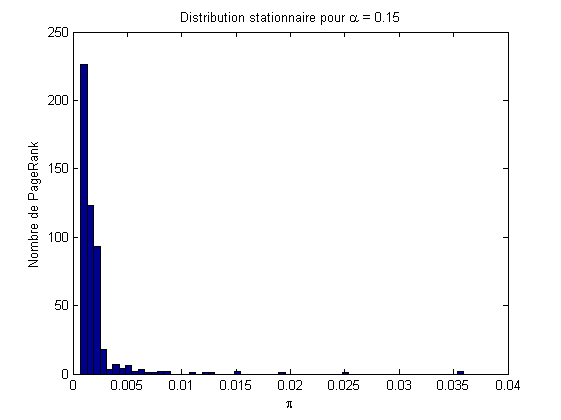
\includegraphics[scale=0.45]{q131_alpha015.png}}
	\subfigure[{$\alpha = 1$}]{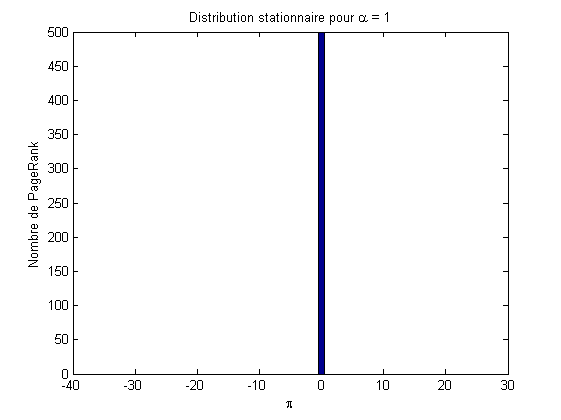
\includegraphics[scale=0.45]{q131_alpha1.png}}
	\caption{Distribution des PageRank lorsque $\alpha$ tend vers 1}
	\label{fig:q131_alpha}
\end{figure}
\end{document}
